\chapter{Toward Write Efficiency and Endurance in SSD RAID}
\chaptermark{TWEEN}
\label{chap:tween}

We thus far focus on tackling small random writes in an erasure-coded clustered
storage. We now introduce another project called TWEEN, which tackles small
random writes in the context of an SSD RAID. In this chapter, we give an
overview of the partial-write problem in SSD RAID and describe the design of
TWEEN.

\section{Partial Writes in SSD RAID}
\label{sec:partial}

\begin{figure}[t]
\centering
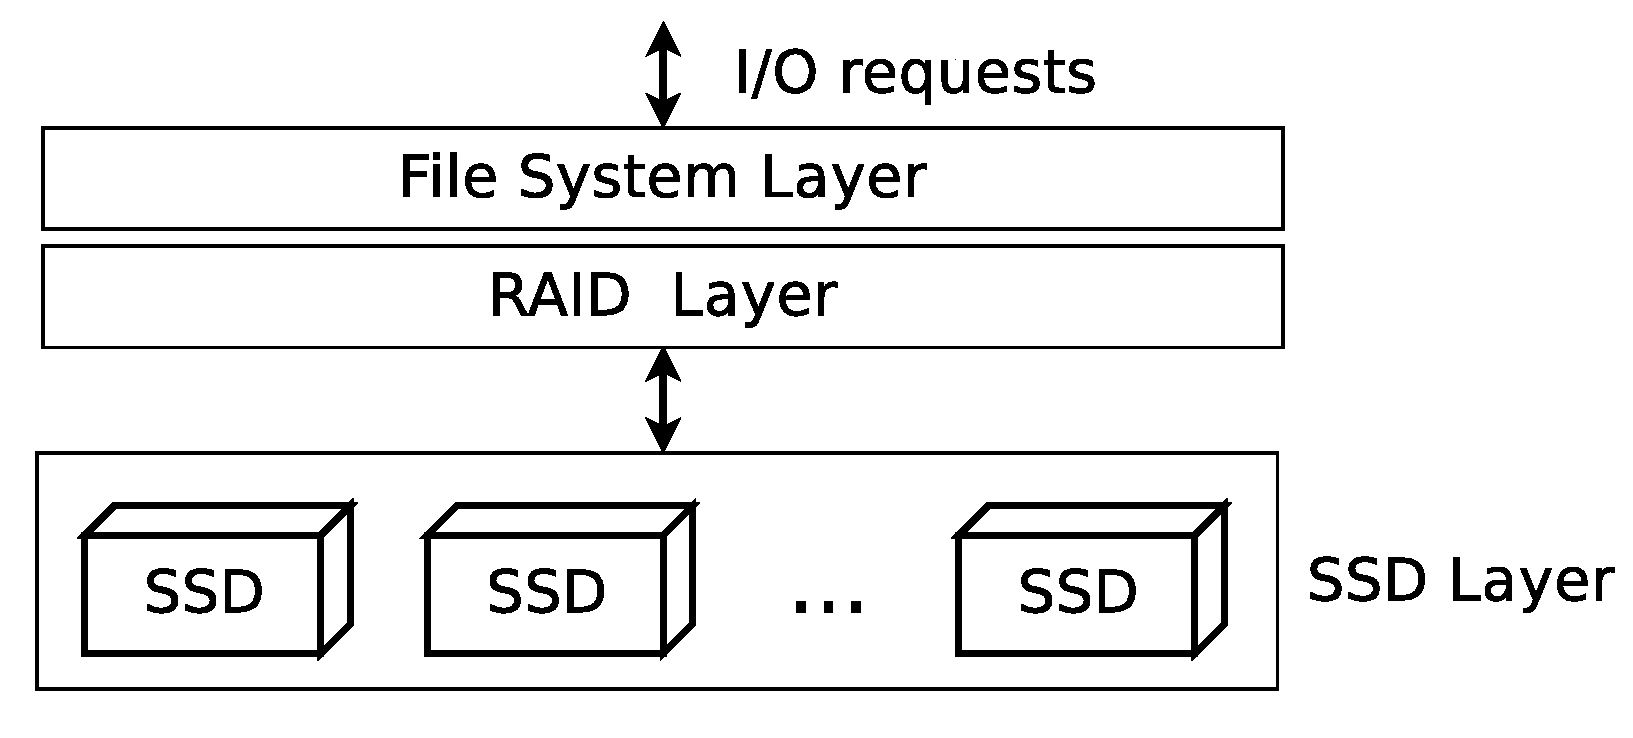
\includegraphics[width=0.7\linewidth]{figs/typical_raid}
\caption{The SSD RAID layout considered in TWEEN.}
\label{fig:typicalraid}
\end{figure}

Small random writes are detrimental to both SSD performance
\cite{kim08,chen09,min12} and RAID performance \cite{stodolsky93}.  They exhibit
in many real-world workloads including those in online transaction-processing
(OLTP) systems \cite{wong02}, desktops \cite{harter11} and enterprise servers
\cite{kavalanekar08}. Also, modern databases and critical applications tend to
call \texttt{fsync/sync} frequently to force {\em synchronous writes}, which
cause writes to be relatively small and random \cite{harter11}.
	   
%partial-stripe writes frequently.  Moreover, recent studies show that random
%writes commonly occur in both enterprise \cite{chan14} and desktop
%\cite{harter11} workloads.  Also, 
	
This section considers two specific types of small random writes that can happen
in an SSD RAID, namely {\em partial-block writes} and {\em partial-stripe
    writes}, whose request sizes are too small and do not align with the
granularities of the SSD and RAID operations, respectively. We collectively call
them {\em partial writes}, which incur performance overhead to SSD RAID as
described below.  Figure~\ref{fig:typicalraid} shows the SSD RAID layout that we
consider in TWEEN.

%\subsection{Partial-Block Writes} 

%Partial writes introduce performance overhead to an SSD RAID.  We classify
%partial writes into \textit{partial-stripe writes} in RAID and
%\textit{partial-block updates} in SSDs. In RAID, partial-stripe writes refer to
%writes that cover only part of a stripe. While these writes are handled using
%either read-modify write or reconstruct write in a parity-based RAID, both
%require extra read operations for maintaining parity consistency.  In SSDs,
%\textit{partial-block updates} refer to writes that change a portion of pages
%in a block. Partial-block updates hinder garbage collection performance and
%shorten the lifetime of SSDs as they tend to fragment a block with live and
%stale pages.

%Figure~\ref{fig:typicalraid} shows a typical SSD RAID setup.  Partial writes
%can occur in either (or both) the (1) SSD layer and the (2) RAID layer.  Our
%goal is to eliminate both partial-stripe writes and partial-block updates
%\textit{on the write path} to achieve optimal update performance and enhance
%SSD lifetime.  
%In this section, we separately study the causes and impacts of the two kinds
%of partial writes and propose a novel file system layer that couples NVRAM
%with a log-structured design as solution.

%\paragraph{When do they happen} 

\subsection{Partial-Block Writes}

In the SSD layer, partial-block writes are the writes that update only a
portion of pages in an SSD block.  Because of out-of-place writes in SSDs
\cite{agrawal08}, 
partial-block writes eventually cause SSD blocks to
contain a mix of live and stale pages, leading to internal fragmentation
\cite{chen09}.  Such internal fragmentation increases the write amplification
overhead of garbage collection, because each time garbage collection needs to
copy many live pages from the chosen block to a free block. If the number of
stale pages in a block is small, then live pages of multiple blocks need to be
relocated so as to reclaim a block that is full of clean pages. Note that the
large write amplification overhead is seen regardless of the underlying
address mapping schemes in FTL \cite{min12}. 

%In an SSD RAID, we see that partial-block updates occur if the RAID layer
%issues write requests that are either (1) unaligned to block boundaries or
%(2) having write size smaller than a block. Typically, the SSD controller
%handles partial-block updates by writing the new data to a clean block and
%marking the original pages as \textit{stale}.

%\paragraph{Why are they harmful} 

%The impacts of partial-block updates are two-fold. First, modern SSDs adopt
%interleaving techniques to boost I/O performance. Large writes spanning across
%multiple pages are inherently faster than small writes. Writes in
%multiples of the \textit{clustered page} \cite{kim12toc} size achieve better 
%I/O performance as they can write to multiple NAND flash chips in parallel.

%\red{[write size vs throughput experiment]}

%However, the fragmentation of live and stale pages in blocks eventually leads
%to write amplification. For page-level mapping FTLs, garbage collection
%suffers from large copying overhead as the controller needs to migrate live
%pages from the victim block to another clean block. For hybrid mapping FTLs,
%garbage collection is likely to trigger the expensive \textit{full merge}
%\cite{gupta09} which copies live pages from both the log blocks and data
%blocks. In either case, write amplification occurs as a result of the
%NAND flash chips receiving extra page writes due to partial-block
%updates.

%\red{[write amplification experiment]} \\

%\paragraph{Solution} 

%One intuitive approach to eliminate partial-block updates is to let the RAID
%layer align writes to the SSD block boundary before issuing them.  For
%page-level mapping FTLs, this eliminates copying overhead in garbage
%collection as all pages in a SSD block are either stale or live.  For hybrid
%mapping FTLs, garbage collection becomes a series of efficient \textit{switch
%merge} \cite{gupta09} operations since one can just replace a data block
%of stale pages with its corresponding log block.  However, the alignment
%operation is costly because it often enlarges the write size by first
%reading data to pack the unaligned writes.

\subsection{Partial-Stripe Writes}

%\paragraph{When do they happen} 

Partial-stripe writes are the writes whose request sizes are smaller than the
size of a stripe in RAID.  Depending on the write size, RAID handles a 
partial-stripe write based on one of the two approaches \cite{chen95}: (1)
\textit{read-modify write} and (2) \textit{reconstruct write} (see
Section~\ref{sec:parity_background}).  Both
reconstruct writes and read-modify writes are inferior in performance as they
incur extra reads before writes.  Instead, it is more desirable to issue 
{\em full-stripe writes}, which incur no read by updating all chunks in a stripe 
and are the most efficient type of writes in RAID \cite{chen95}. 

%Typically, workloads dominated by small and random writes such as those from
%online transaction-processing (OLTP) systems \cite{wong02} tend to trigger
%partial-stripe writes frequently.  Moreover, recent studies show that random
%writes commonly occur in both enterprise \cite{chan14} and desktop
%\cite{harter11} workloads.  Also, modern databases and critical applications
%tend to call \texttt{fsync/sync} frequently to force writes to disk, which
%cause writes to be relatively small and random \cite{harter11}.

%\paragraph{Why are they harmful} 

%\paragraph{Solution} 

%However, while this improves user experience, it only delays does not work well
%under intensive workload once the NVRAM is exhausted \red{[CITE]}.

%Intuitively, a log-based design converts small random writes to large
%sequential writes through batching. Updates are packed in a log until there
%are sufficient data to issue a full-stripe write~\cite{menon95}.  Although a
%log-based design eliminates read operations on the write path, the garbage
%collection mechanism requires careful consideration as it is known to hinder
%system performance~\cite{seltzer95}.


\section{TWEEN Design}
\label{sec:design}

We propose TWEEN, a middleware application that aims \underline{t}oward
\underline{w}rite \underline{e}fficiency and \underline{en}durance in SSD
RAID.  TWEEN comprises two key technologies.  It couples LFS and NVRAM, by
batching partial writes in NVRAM buffers and issuing only large writes to SSD
RAID.  Also, it mitigates the garbage collection overhead in LFS by grouping
writes with similar file access frequencies and absorbing garbage collection
writes in NVRAM.  In this section, we elaborate the design details of
TWEEN and justify how this design addresses the partial-write problem in SSD
RAID.  
%It is motivated by two design principles: (1) minimizing the garbage
%collection overhead of SSDs due to partial-block writes and (2) minimizing
%the parity update overhead of RAID layer due to partial-stripe writes.
%%(i.e., using full-stripe writes only).   


\subsection{Goals}

We first present our design goals.
\vspace{-3pt}
\begin{itemize} \itemsep=1pt
\item {\bf Write efficiency and endurance:}  Given the partial-write problem
(see \S\ref{sec:partial}), TWEEN aims to optimize both
write and garbage collection flows by eliminating partial-block writes and
partial-stripe writes at SSD and RAID levels, respectively.  
See \S\ref{subsec:key} and \S\ref{subsec:architecture}. 
\item {\bf Metadata efficiency:}  TWEEN maintains metadata to manage the write
and garbage collection flows.  It is critical that the metadata overhead is
limited compared to the actual data storage.  See \S\ref{subsec:metadata}.
\item {\bf Availability:}  TWEEN should preserve device-level fault tolerance
offered by SSD RAID. Also, the data consistency between TWEEN and the underlying
SSD RAID should be maintained. See \S\ref{subsec:availability}.  
% TWEEN can be inconsistent with underlying RAID when write hole happens
\item {\bf Compatibility:}  When optimizing the write efficiency and endurance
of SSDs, RAID, or the integration of SSD and RAID, previous studies 
focus on modifying either SSD or RAID
controllers.  However, modifying SSD or RAID controllers often requires
extensive engineering work.  Thus, when we design TWEEN, it should be
compatible with off-the-shelf SSD RAID configurations.  
See \S\ref{subsec:implementation}.
%We note that previous studies also adopt the LFS design to improve RAID
%performance, they focus on applying logging in the RAID layer. A new RAID
%implementation requires re-engineering of RAID controllers
%\cite{menon95,wilkes95}, and this is often infeasible for hardware RAID.  In
\end{itemize}


\subsection{Key Technologies}
\label{subsec:key}

We elaborate two key technologies of TWEEN to achieve our design goals: (1)
eliminating partial writes and (2) mitigating the LFS garbage collection
overhead. 

\subsubsection{Eliminating Partial Writes}
\label{subsubsec:eliminating}

The core design of TWEEN is the log-structured file system (LFS)
\cite{rosenblum92} coupled with byte-addressable non-volatile RAM (NVRAM) buffering.  
TWEEN follows LFS \cite{rosenblum92} by batching incoming small writes
sequentially and flushing them to SSD RAID when the aggregated write size
aligns the unit sizes of RAID encoding and SSD garbage collection. 

%Partial writes introduce parity update overhead in RAID and slow down GC in
%SSDs. 

TWEEN batches partial writes in buffers.  In this work, we choose NVRAM-based
buffering, and take advantage of the low-latency and persistence properties of
NVRAM.  NVRAM has emerged to be a potential candidate for substituting DRAM in
computer systems due to its lower energy consumption and persistence
properties \cite{zhou09,lee14}.  We consider byte-addressable NVRAM such as
PCM (phase-change memory), FRAM (ferro-electric RAM), STT-RAM
(spin-transfer torque RAM) and NVDIMM (non-volatile DIMM).  While these variants differ in capacity,
performance and endurance \cite{jung10}, they all offer better performance and
endurance than flash.  For example, the write latency for PCM is
\SI{180}{\nano\second}, as opposed to \SI{200}{$\mu$\second} for NAND flash
\cite{jung10}.  Also, PCM and
STT-RAM can sustain more than $10^7$ and $10^{15}$ rewrites per cell,
respectively \cite{jung10,zhou09}. NVDIMM has recently
emerged as a new type of NVRAM which provides the same speed and endurance as DRAM,
and can be seamlessly integrated in existing DDR3 architecture \cite{viking}.
Previous studies have extensively studied
the use of NVRAM in storage systems to improve performance and reliability
%\cite{wang06,jung10,venkataraman11,zhou09,qiu13,lee14}.  
\cite{jung10,venkataraman11,zhou09,qiu13,lee14}.  

%(1) Unlike flash where writes are in pages, NVRAM provides a byte-addressable
%interface. (2) There is no need for NVRAM to erase a block before updating
%it, which often hinders performance in flash. (3) NVRAM offers significantly
%lower write latency: \SI{180}{\nano\second} for PCM as opposed to
%\SI{200}{\micro\second} for flash \cite{jung10}.  (4) NVRAM has substantially
%better endurance than flash. For example, PCM and STT-RAM cells can sustain
%more than $10^7$ and $10^{15}$ rewrites per cell respectively
%\cite{jung10,zhou09}.  Recent trends have shown that the density and
%endurance of NVRAM can be further improved using techniques like multi-level
%designs and 3D die stacking techniques \cite{venkataraman11}. Despite the
%current high cost, 

TWEEN keeps multiple NVRAM buffers, each of which corresponds to a hotness
group (see \S\ref{subsubsec:mitigating}). It associates each NVRAM buffer with
a \textit{segment}, which is the aggregate of multiple partial writes.  Each
segment has the same size as a RAID stripe and is the minimum flush unit in
TWEEN.  TWEEN only issues full-stripe writes to SSD RAID so as to avoid
reading old data and parity chunks as seen in partial-stripe writes.  This reduces the
parity update overhead.  Also, by setting the RAID chunk size to be a multiple
of the SSD block size, TWEEN simultaneously eliminates partial-block writes in
each SSD. 

% PC: this part is to be explained in the next subsection
%Each write is appended to one of the segments based on its hotness group (see
%\S\ref{sec:hotmod}).  When a segment is fully filled with data, it is
%sealed and flushed to SSD RAID with a full-stripe write (i.e., writing all
%data and parity chunks of a stripe).  Afterwards, TWEEN reuses the
%buffer by associating it with a new segment.  

Compared to typical hardware RAID controllers (e.g., \cite{dell,lsi}) which
treat NVRAM merely as a write-back cache, TWEEN introduces NVRAM as an extra
tier of storage for keeping partially written segments.  The persistence
nature of NVRAM allows TWEEN to efficiently handle \texttt{fsync/sync}
commands issued by upper-layer applications and avoid issuing partial writes
to storage. 

%TWEEN eliminates partial writes to SSD RAID by batching them using LFS and
%NVRAM.  We address the following two issues as a result of the design.

TWEEN uses only a small amount of NVRAM.  Recall that each NVRAM buffer is
configured to have the same size as a RAID stripe.  Our default configuration
of TWEEN uses the \SI{8}{MB} stripe size and four NVRAM buffers, accounting for
\SI{32}{MB} of NVRAM in total.  Note that the configured NVRAM capacity is
independent of the total amount of data written to SSD RAID.  In addition,
TWEEN stores all metadata in NVRAM for simplicity and performance.  We show
the metadata only occupies a limited amount of NVRAM in the worst case (see
\S\ref{subsec:metadata}) and under real-world workloads. 
%although keeping most of the metadata on the SSDs is also feasible by
%utilizing data structures like B-Tree. Nevertheless, 
%We pose the issues of further reducing NVRAM capacity requirements as future work.

TWEEN offloads garbage collection from SSDs to the LFS layer by always writing
in units of blocks (i.e., avoiding partial-block writes). However, the garbage
collection overhead still exists in TWEEN
, as it is now moved to the LFS layer.  
The LFS garbage collection is known to hamper I/O performance by (1)
introducing copying overhead \cite{seltzer95} and (2) causing I/O contentions
\cite{shin13}.  We address this issue in the following discussion. 

\subsubsection{Mitigating LFS Garbage Collection Overhead}
\label{subsubsec:mitigating}

TWEEN eliminates partial writes using the LFS design, and hence it needs to
address garbage collection in the LFS layer.  Here, we propose two
workload-aware approaches to mitigate the LFS garbage collection overhead.

First, TWEEN exploits workload characteristics to reduce copying overhead of
garbage collection.  It has been known that writes in real-world workloads are
non-uniform and have different update frequencies \cite{min12,zhang13}. 
%exhibit spatial and temporal localities in data accesses \cite{zhang13}. 
Thus, TWEEN continuously monitors the update frequency of each file and
assigns a \textit{hotness} value to each file. We pack writes with similar
hotness in the same segment using a simple clustering algorithm (see
\S\ref{subsubsec:hotmod}).  The intuition is that hot segments are frequently
updated and hence likely contains stale data, while cold segments are likely
occupied with live data.  TWEEN greedily garbage-collects hot segments with
most stale data to minimize the amount of data reclaimed.  

%As data with similar hotness tends to be updated at roughly the same time,
%our approach effectively increases the number of all-stale and all-live
%segments in the system \red{[need a better and more accurate
%description...forms a bimodel distribution?  pushes distribution of
%data in a segment towards all-live and all-stale?]}.  

%We discuss the hotness grouping algorithm and GC procedures in detail in
%\S\ref{sec:hotmod} and \S\ref{sec:gcmod}, respectively.

%Since TWEEN logs updates in the file system layer instead of in the RAID layer,
%it calculates a \textit{hotness} value for each writes to perform grouping
%based on file-level information including the update frequency. 

%In addition, when we use LFS on top of RAID, the need for updating parity adds
%extra cost to garbage collection.  While the idea of using a log-structured
%scheme for RAID is not new, previous studies focus on logging in the RAID layer
%\cite{menon95,wilkes95}.  We observe that logging in the file system layer
%allows us to exploit file-level information including the update frequency and
%locality. We use this information to perform hotness grouping \textit{on the
%write path}. Every write is assigned to a segment according to the popularity
%(or hotness) of its file. As data with similar hotness are typically updated
%and marked stale at roughly the same time, this approach increases the number
%of all-stale or all-live segments and speeds up garbage collection in the file
%system layer as a result. We discuss the hotness grouping algorithm in detail
%in \S\ref{sec:hotmod}

Second, when TWEEN reclaims live data during LFS garbage collection, it
returns the reclaimed data back to NVRAM buffers instead of writing the data
directly to SSD RAID.  
%Thus, we ensure that the only writes to SSD RAID are
%issued by the segment writes from NVRAM buffers.  
This prevents LFS garbage
collection itself from issuing partial writes to SSD RAID and contending with
normal user writes.  Also, this provides a feedback mechanism to re-assess
the hotness of the reclaimed live data after LFS garbage collection, which may
have different update frequencies.  Such {\em iterative} hotness grouping can
improve the accuracy of workload characterization.  
%We evaluate the effectiveness of this iterative hotness grouping mechanism in
%\S\ref{eval:hotness}.

The number of hotness groups affects the clustering accuracy, which is
directly related to the garbage collection performance in TWEEN. Using too
many hotness groups may lead to \textit{over-fitting}, in which noises in
samples lower the clustering accuracy; on the other hand, using too few groups
may also affect clustering accuracy due to coarse-grain classification. 
%parallelism in the log module.  , because the number of NVRAM log buffers is
%equal to the number of hotness group. 
Choosing the right number of hotness groups is non-trivial and highly
dependent on the target workload. 
%We evaluate the effectiveness of different hotness group settings in real-world scenarios.

\subsection{Architecture}
\label{subsec:architecture}

We now describe the internal architecture of TWEEN and explain how it
realizes the aforementioned technologies.  TWEEN focuses on optimizing both
write and garbage collection flows.  It uses the same read flow as the
conventional LFS, and we omit the details here. 

\begin{figure}[t]
    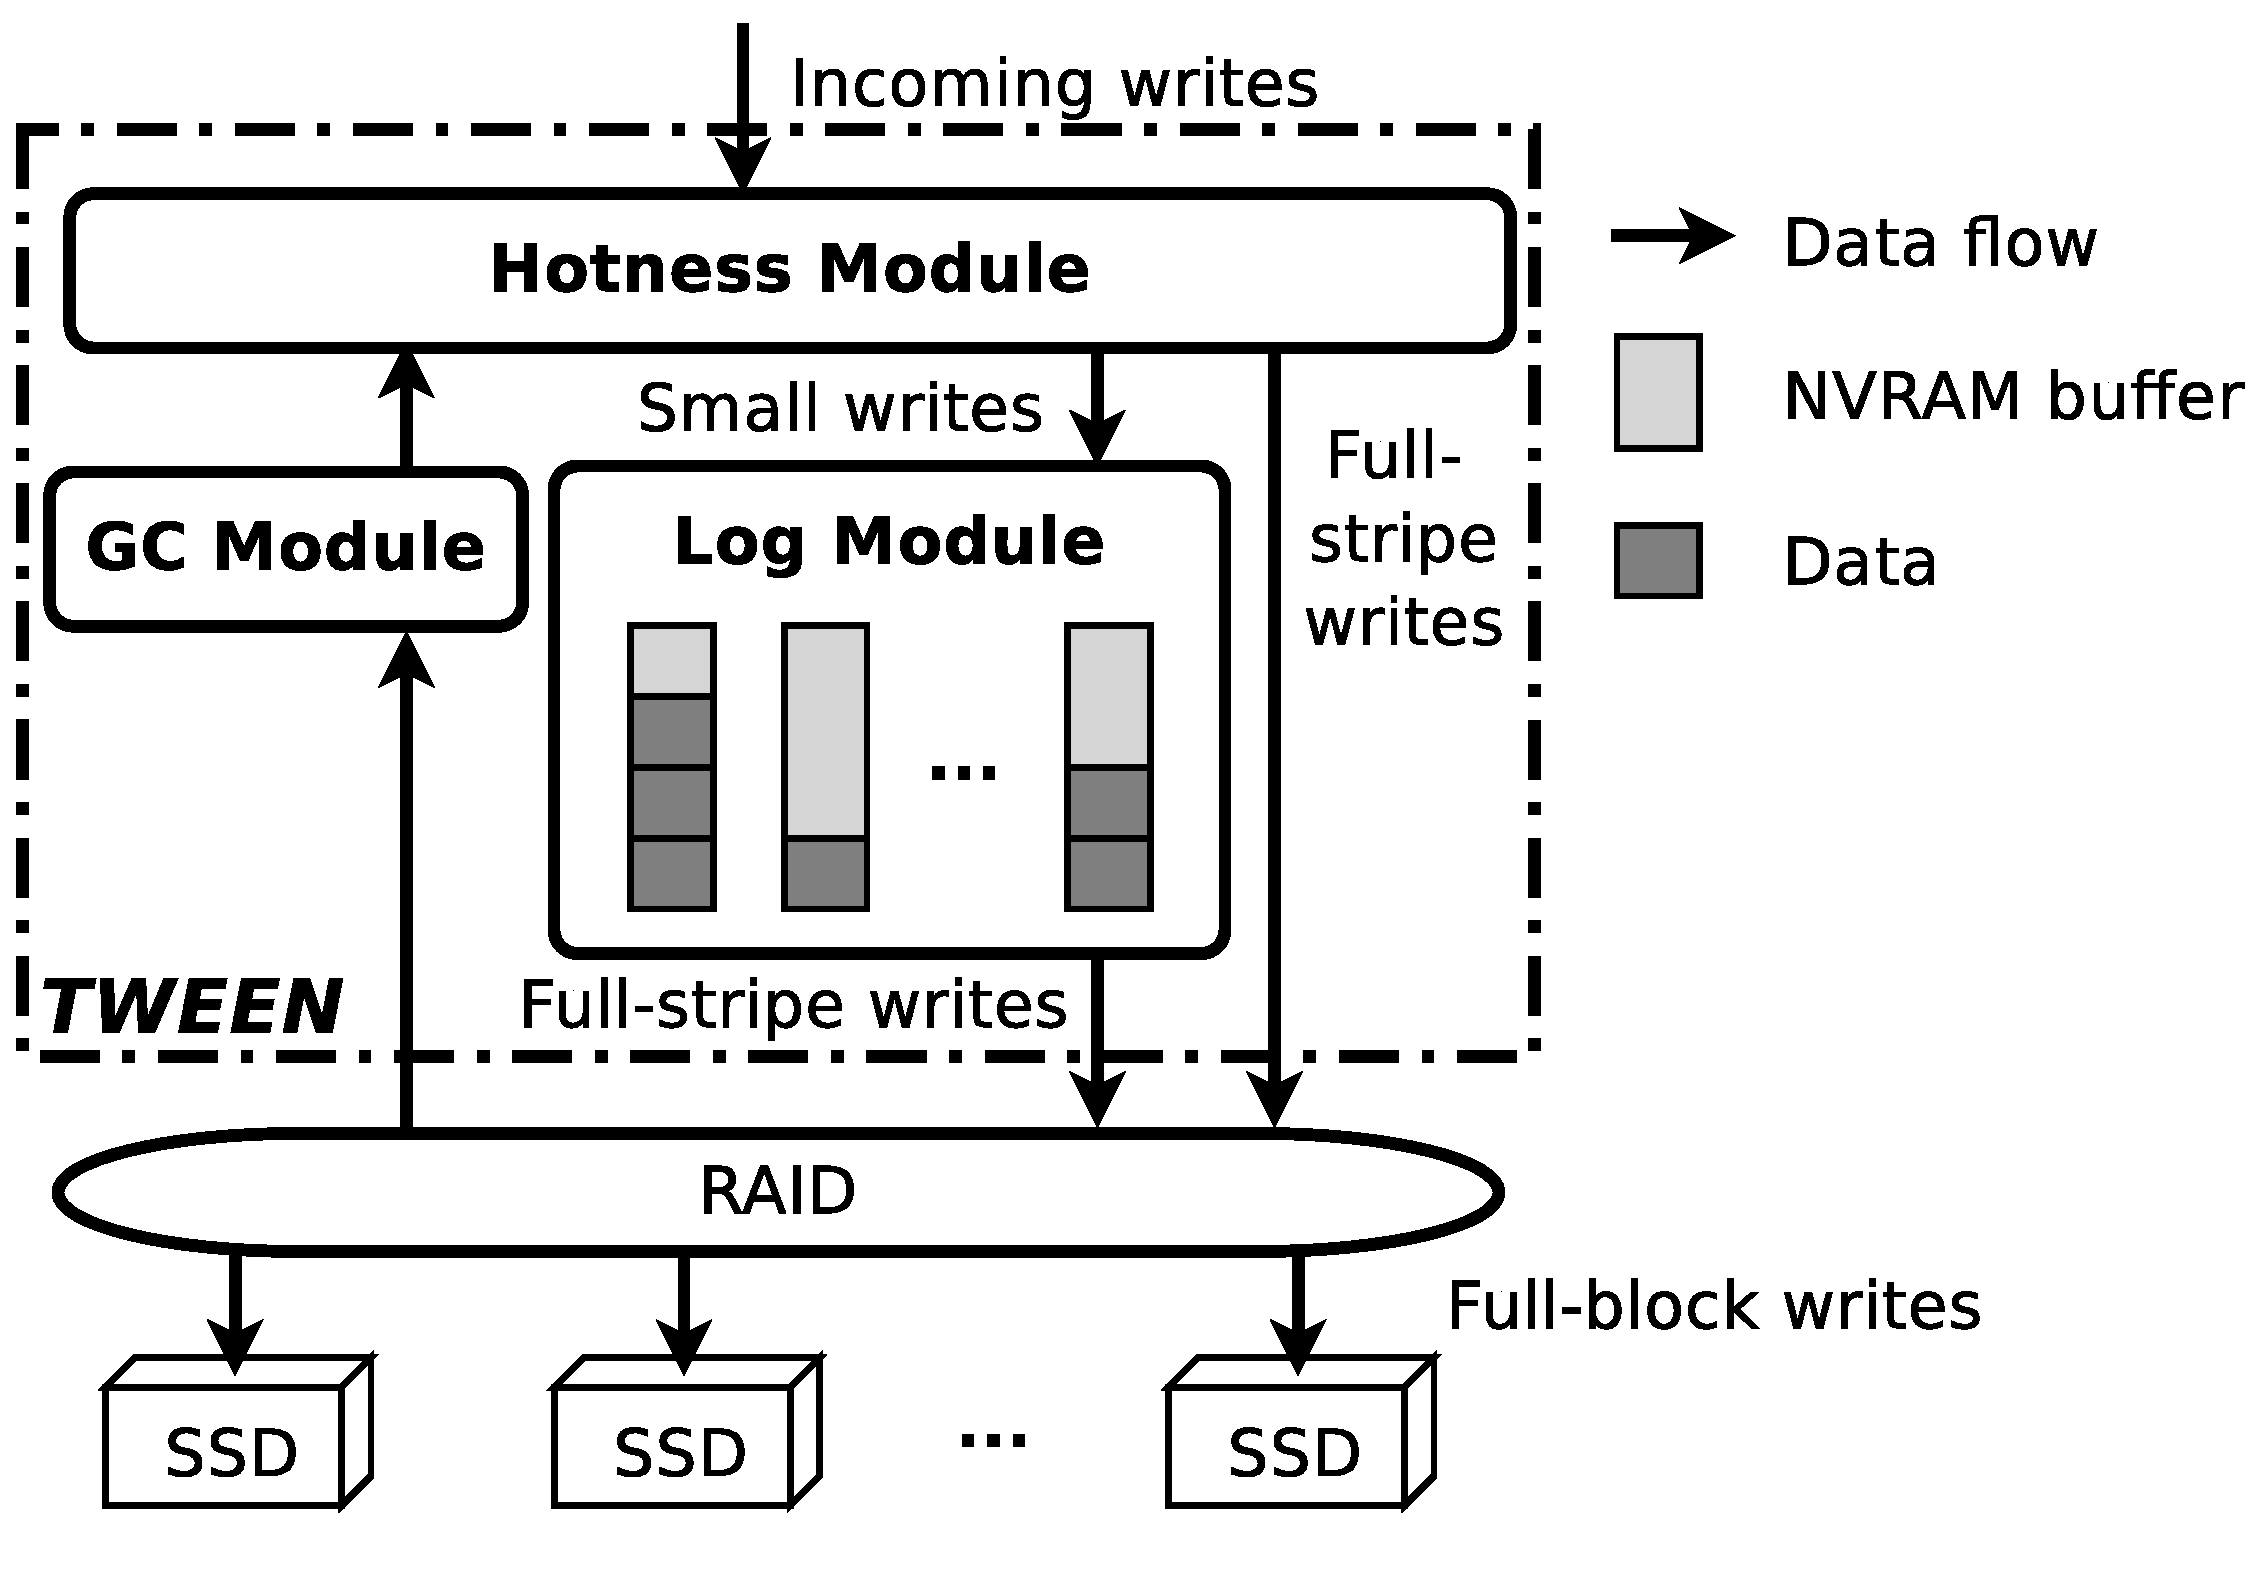
\includegraphics[width=0.99\linewidth]{figs/ssdraid_arch_2}
    %\vspace{-3pt}
    \caption{TWEEN architecture.}
    \label{fig:architecture}
\end{figure}

Figure~\ref{fig:architecture} shows the TWEEN architecture, which consists of
three major modules. The \textit{hotness module} manages system metadata,
monitors the update frequency of each file, and assigns a hotness group to
each write based on the file's hotness value.  The \textit{log module} handles
the write flow.  It maintains an NVRAM buffer for each hotness group. Each
buffer batches writes until a segment is full and can be flushed to the
SSD RAID as a full-stripe write. Recall that the chunk size is set to be 
a multiple of SSD block size. Each full-stripe write results in full-block writes to the
SSDs.  The \textit{garbage collection (GC) module} reclaims space 
from stale segments by reading segments from the SSD
RAID and sending live data back to the hotness module. In the following, we describe the
design details of each module. 

\subsubsection{Hotness Module}
\label{subsubsec:hotmod}

The hotness module keeps track of each file's hotness value, denoted by
$H_{f}^{t}$ of each file $f$ at time $t$.  The hotness value captures the
update frequency of a file over time. 
%Alternatively, $H_{f}^{t}$ can be interpreted as the \textit{update likelihood}
%of file $f$ as it represents the chance that the file will be updated at the
%next time interval. 
We calculate $H_{f}^{t}$ using an exponential moving average approach:
$$
H_{f}^{t} = \alpha\frac{1}{t-\hat{t}} + (1-\alpha)H_{f}^{\hat{t}}
$$
where $\hat{t}$ denotes the last modified time of file $f$ and 
$\alpha$ is a smoothing factor.

To determine the hotness group of a particular file, the hotness module 
performs data clustering based on the hotness values of all files and selects
one cluster which is closest to the file in question as its hotness group. As
classification is performed for every write, the hotness module adopts the
efficient sequential $K$-means clustering algorithm \cite{macqueen67} to
minimize computational overhead.

Algorithm~\ref{alg:kmean} describes the hotness classification mechanism.
Here, the user specifies the number of hotness groups $N$.  During startup, we
make initial random guesses for the cluster centers.  Next, for each
classification query, we find the closest center using the \texttt{diff(x,y)}
function, which computes the absolute difference between a query $H_{f}^{t}$
and a center $C_{i}$ for the $i$-th cluster (where $1\le i\le N$).  Upon
selecting a center $C_i$, we update the center value with an aging factor
$\beta$ and return the query answer.

%Such iterative center update introduces
%minimum overhead to write opeartions
%We note that the classification overhead is
%independent of the number of files in the system as we use only the cluster
%centers for each classification.

\begin{algorithm}[t]
    \small
    \DontPrintSemicolon
    $N \gets $\verb|HOTNESS_GROUP|\;
    Make initial guesses for the cluster centers $C_{1}, C_{2},...,C_{N}$ \;
    \While{$\rm{true}$}{
    Acquire the next classification query, $H_{f}^{t}$ \;
    \If{\FuncSty{diff}$(C_{i}, H_{f}^{t})$ \emph{is smallest among all centers}} {
    $C_{i} \gets C_{i} + \beta(H_{f}^{t}-C_{i}) $\;
    Classify $H_{f}^{t}$ as hotness group $i$\;
    }
    }
    \caption{Hotness clustering and classification}
    \label{alg:kmean}
\end{algorithm}

The hotness value as well as other file system metadata are kept in NVRAM for
performance and reliability reasons, as both types of data are frequently
accessed and updated.  We examine the metadata overhead in
\S\ref{subsec:metadata}.
%We minimize the size of metadata by storing only the
%necessary information including the hotness values, 
%the file-to-segment mapping tables and on-disk locations of segments.

\subsubsection{Log Module} 

The log module maintains $N$ NVRAM buffers for logging writes, where $N$ is
the number of hotness groups.  Each buffer holds a segment for each hotness
group, and the segment size is set to be the same as the RAID stripe size.
The NVRAM buffers also act as non-volatile cache and serve read requests for
data that is not yet flushed to the underlying SSD RAID.

%To ensure writes with similar hotness can be batched together, the number of
%pre-allocated buffers is equal to the number of hotness groups. 
%\red{We use replication to make the logging module achieve the same fault tolerance
%    level as the RAID configuration.}

Each incoming write is first handled by the hotness module, which updates the
file hotness and assigns a hotness group for the write. If the write size is
larger than a stripe, the hotness module can bypass logging by issuing
full-stripe writes to SSD RAID until the remaining data is insufficient to fill 
a stripe. Next, the log module receives the data from the hotness module after
classification and appends the write to the corresponding NVRAM buffer.  If
the buffer is full, the log module seals and flushes the segment to SSD RAID
by issuing a full-stripe write.  It then clears the buffer and associates it
with a new segment. Finally, the log module acknowledges the hotness module
on metadata updates.

\subsubsection{Garbage Collection (GC) Module}
\label{subsubsec:gcmod}

%We offload garbage collection from SSDs by performing cleaning operations on
%a segment basis in the file system layer.  

%Because the logging module uses NVRAM for storage, the cost of
%cleaning, which is only one read from the RAID, is identical for any segment.
%Hence we can choose the cleaning target by greedily choosing the one that can
%free maximum space.

The GC module cleans stale segments to reclaim space.  We design the GC module
to be aware of the file update frequency by coupling it with the hotness module.
In each garbage collection operation, the GC module reads the entire
garbage-collected segment and reclaims live data within.  It then sends the
remaining live data of each file back to the hotness module, which re-classifies
and directs data to the log module. It frees the address of the reclaimed
segment by updating the corresponding metadata entry.

TWEEN supports two garbage collection modes: (1) \textit{periodic} and (2)
\textit{active} \cite{rosenblum92}.  Periodic mode reclaims space from stale
data during system idle time in the background, while active mode reclaims
space when the total storage space including both live and stale data
exceeds some threshold.  For more write-intensive workloads, active mode is
preferred over periodic mode as the idle time between requests is short.
%, at the expense of higher garbage collection overhead.  
In our evaluation, we choose one of the two modes depending on the
workloads we consider. 

%utility grows beyond a certain threshold $t_u$, even though the GC operations
%may stall normal writes and degrade system performance. Here, we define the
%storage utility as the ratio of the storage amount used in TWEEN to the
%amount used in an overwritten file system. The active GC keeps reclaiming
%space until a sufficient number of clean segments is available in the system.

%However, choosing a suitable threshold remains an open issue and 
%requires careful considerations.  Setting a low threshold may result in 
%frequent GC operations; while a high threshold may stall normal writes for a
%long time.
%to take a long time.

%TWEEN utilizes both periodical GC and active GC. For active GC, we define the
%storage utility ratio as the ratio of total physical space used in SSDs to the
%total logical size of files stored. We then set $t_u$ as the threshold of the
%utility ratio \red{[way to determine $t_u$?]}.  TWEEN triggers active GC once
%the storage utility ratio grows beyond $t_u$ and continues until a sufficient
%number of clean segments is available in the system.


%telling the RAID that the entire

%% JEREMY: "how does hotness work" is already explained in "Our Approach"

%the unnecessary data written back for cold data
%during garbage collection, because the segments with cold data contains too few
%stale data to be chosen as cleaning targets.

%\subsection{Data Flow}
%
%The data flow for reads is straightforward in TWEEN. 
%The hotness module directs a read operation to the log module if
%the data is currently residing in the NVRAM buffer or to RAID
%if the data is on the SSDs. We utilize the existing read-ahead 
%mechanism in the Linux kernel to boost read performance.
%We now describe the data flow for writes.

%\subsubsection{Normal Write} 
%
%Each incoming write is first handled by the hotness module, which updates the
%file hotness and assigns a hotness group for the write. If the write size is
%larger than a stripe, the hotness module can bypass logging by issuing
%full-stripe writes to RAID until there is not enough remaining data to fill a
%stripe. Next, the hotness module sends the data to the log module for
%classification, which appends
%the write to the corresponding NVRAM buffer.  If the buffer
%is full, the log module flushes the data to RAID by issuing a full-stripe write
%and clears the buffer. Finally, the hotness module updates the metadata and
%acknowledges the write to the application.

%Upon success, the logging module acknowledges the write finished.
%Otherwise, before sending acknowledgment, the logging module fills 
%the buffer with part of the write to issue a full segment write and 
%clears the buffer to append the remaining part. Finally the hotness
%module receives all the acknowledgments and updates the file and segment metadata 
%for the write.

%\subsubsection{GC Write}
%
%The GC module chooses victim segments to clean base on the amount of
%stale data inside. Once a victim is chosen, the GC module reads the
%entire segment from RAID and drops the stale data. The GC module 
%separates the live data by file and sends the data back to the hotness module,
%which handles these writes like normal writes.
%Finally, the GC module frees the address of the reclaimed segment by updating
%the corresponding metadata entry.

%telling the RAID that the entire
%segment is useless. Thus the RAID knows that the segment's address is free to
%use.

\subsection{Metadata Management}
\label{subsec:metadata}

%In this section, we study the NVRAM usage of our design. We use NVRAM to 
%batch small writes in the logging module and keep all file and 
%segment metadata in the hotness module. We formulize the usage of 
%NVRAM and show that our system only requires moderate NVRAM under common settings.
%The notation in the following discussion is listed in Table~\ref{tab:notation}.

TWEEN maintains a flat namespace and a set of metadata structures to 
keep track of file information and the locations of updates.  The metadata in
TWEEN can be classified into two types: (1) file metadata and (2) segment
metadata. File metadata stores the file identifier, current hotness value, and
the set of composing segments. Segment metadata stores the segment identity
and its location.  

The total metadata size is determined by different factors, including the size
of the SSD RAID volume and the update pattern.  In the following, we conduct
simple analysis and derive the metadata size under the worst case scenario.
Our goal is to show that the metadata overhead in TWEEN is small and has
limited adverse impact on TWEEN performance.  Table~\ref{tab:notation} shows
the notation used in our analysis. 

%The calculation of NVRAM usage $\mu_{L}$ in the logging module is straightforward. The
%size of NVRAM is equal to the size of pre-allocated NVRAM buffer for each
%hotness group, multiplied by the fault-tolerance level ,
%which can be formulized in \eqref{eqn:nvram_logging}.
%\begin{equation}
%    \label{eqn:nvram_logging}
%    \mu_{L} = N\times(kB)\times m = kmNB
%\end{equation}

We first compute the total size of segment metadata (denoted by $\sigma_{S}$). 
We configure each segment to be the same as the RAID stripe size, whose size
is equal to $K\times B$, where $K$ is the number of data chunks per stripe and
$B$ is the data chunk size.   Thus, $\sigma_{S}$ is calculated as:
\begin{equation}
    \label{eqn:nvram_segment}
	\sigma_{S} = \frac{T}{K\times B} \times
	(\mathrm{SZ}(id)+\mathrm{SZ}(addr)) =
    \frac{16T}{K\times B}
\end{equation}
%
where $\frac{T}{K\times B}$ is the maximum number of segments that the system
can store, and $\mathrm{SZ}(\cdot)$ is a function that returns the variable
size in bytes.

%The lower bound of $\sigma_{F}$ is obtained by
%assuming that a single file covers the entire storage space, and that the file
%is composed of $\frac{T}{KB}$ segments. Then we can
%express:
%\begin{equation}
%    \label{eqn:nvram_filelow}
%    \begin{split}
%    \sigma_{F} &\ge \frac{T}{KB} \times \mathrm{SZ}(\varphi_{f}) +
%    \mathrm{SZ}(i_{f}) + \mathrm{SZ}(s_{f}) + \mathrm{SZ}(H_{f}) \\
%    &= \frac{20T}{KB} + 20 
%\end{split}
%\end{equation}

We next compute the total size of file metadata (denoted by $\sigma_{F}$).
Since $\sigma_{F}$ depends on the file size distribution, we compute its upper
bound.  This happens when the entire storage space is covered with files whose
sizes are the same as the read/write unit size (e.g., an SSD page size).  We
obtain $\sigma_{F}$ by summing the size of the file metadata of each file $f$
as follows:
%
\begin{equation}
    \label{eqn:nvram_fileup}
    \begin{split}
    \sigma_{F} &\leq  \sum_{f} (\mathrm{SZ}(\varphi_{f}) +
    \mathrm{SZ}(i_{f}) + \mathrm{SZ}(s_{f}) + \mathrm{SZ}(H_{f}))  \\
    &= \frac{T}{S} \times( \mathrm{SZ}(\varphi_{f}) +
    \mathrm{SZ}(i_{f}) + \mathrm{SZ}(s_{f}) + \mathrm{SZ}(H_{f})) \\
    &= \frac{40T}{S}
\end{split}
\end{equation}

Finally, we express the upper bound of the total metadata size as a percentage
$\rho$ of the storage capacity: 
%
\begin{equation}
    \label{eqn:nvram_over}
    \begin{split}
    %\rho &= \frac{\sigma_{S} + \sigma_{F}}{T} \ge \frac{36}{KB} +
    %\frac{20}{T}\\
    \rho &= \frac{\sigma_{S} + \sigma_{F}}{T} \leq 
    \frac{16}{K\times B} + \frac{40}{S}
\end{split}
\end{equation}

Consider a typical SSD RAID configuration with
$K=4$, $B=\SI{512}{KB}$, $S=\SI{4}{KB}$, $T=\SI{1}{TB}$, we have $\rho \leq
0.98\%$, which we believe is reasonable metadata overhead.  The metadata
overhead can be further reduced by using a larger segment size (or RAID
stripe size) and read/write unit. 

%, which is a moderate
%overhead compared to ext4's(\red{need cite}).
\begin{table}[t]
    \centering 
    \small
    \begin{tabular}{|c|c|l|} 
        \hline
        {\bf Notation}  & {\bf Type(bytes)} & {\bf Description}\\ 
        \hline 
        \multicolumn{3}{|c|}{Global Settings} \\
        \hline 
        $T$ & long(8)  & storage capacity for data chunks\\
        %$N$  & int(4) & number of hotness groups\\
        $B$ & int(4) & data chunk size \\
        $K$ & int(4) & number of data chunks per stripe\\
        $S$  & int(4) & read/write unit size\\
%        $m$ & int(4)& fault tolerance level \\
        \hline 
        \multicolumn{3}{|c|}{Metadata of File $f$} \\
        \hline
        $i_{f}$ & long(8) & file identifier\\
        $s_{f}$ & long(8) & file size  \\
        $H_{f}$ & float(4) & hotness value \\
        $\varphi_{f}$ & tuple(20) & file location, $\tuple{long,long,int}$ \\ 
        %$L_{f}$ & set & file location set  \\
        \hline 
        \multicolumn{3}{|c|}{File Location $\varphi_{f} = \tuple{i_{s},o_{f},o_{s}}$} \\
        \hline 
        $i_{s}$ & long(8) & segment identifier\\
        $o_{f}$ & long(8)& file offset \\
        $o_{s}$  & int(4)& segment offset\\
        \hline
        \multicolumn{3}{|c|}{Metadata of Segment $s$} \\
        \hline
        $id$ & long(8) & segment identifier\\
        $addr$  & long(8) & segment location\\
        \hline
    \end{tabular}
    \caption{Notations for metadata structures.}
    \label{tab:notation} 
\end{table}


\subsection{Availability}
\label{subsec:availability}

% the "write hole" refers to the window of vulnerability

TWEEN keeps writes temporarily in NVRAM before flushing them to SSD RAID. Our design
defers RAID protection on the data based on the assumption that NVRAM is a
highly-reliable component in our architecture and keeps data available in the
presence of transient failures (e.g., power loss) \cite{jung10}. 
%In addition,
%it is shown that the degradation of fault tolerance due to deferred parity
%updates is small in practical RAID systems \cite{savage96}. 

%Thus, we sacrifice small
%degradation of fault tolerance for significantly improved write performance. 

However, if a power loss occurs in the middle of a full-stripe write and only
part of a stripe is written to SSD RAID, the parity may become inconsistent with the
data. If SSD RAID uses the inconsistent parity to
reconstruct data, it may lead to data corruption (also known as the write hole
problem \cite{appuswamy10}).
%even the number of device failures is within the level of fault tolerance
%provided by the RAID configuration \cite{appuswamy10}. 
%Researchers refer this phenomenon as the RAID \textit{write hole}
%\cite{appuswamy10} problem.  Data corruption may happen if a disk failure
%occurs at this point and the inconsistent parity is used to reconstruct data.
TWEEN prevents this issue by atomically updating metadata structures 
only after each write is successfully completed in the underlying SSD RAID.
%Suppose that an unclean shutdown results in an inconsistent parity in
%one of the stripes and a subsequent device failure triggers RAID
%reconstruction, which propagates the error to the data chunks. 
Therefore, the metadata structures in TWEEN always present a consistent
version of the file system to read requests. 
%We note that there is no need to
%explicitly handle the currently inconsistent stripe in RAID since the write is
%already discarded and TWEEN will overwrite the location with a new stripe
%eventually. {\bf PC: double check???}

\subsection{Implementation Details}
\label{subsec:implementation}

We build TWEEN entirely as a user-space application, and hence it is
compatible with off-the-shelf RAID (including its hardware and software RAID
variants) and SSDs.   We implement the TWEEN prototype in C++ on Linux.  The
TWEEN core implements all the software modules described in
\S\ref{subsec:architecture}.  It has around \num{2400} lines of code
in total. 

Our TWEEN prototype exports the file system interface as a client API
that allows upper-layer applications to access the underlying SSD RAID through
TWEEN.  The API supports the essential file system operations for our
performance evaluation, such as creating, reading, and writing files.  Since
TWEEN supports the basic file system functionalities, we can compare it with 
state-of-the-art file systems.  Nevertheless, our
current prototype does not support all file system features such as
permissions and security.  We pose the full file system implementation as
future work.



\section{Summary}

We propose TWEEN, a middleware application designed to enhance the write
efficiency and endurance of SSD RAID. TWEEN has several design goals: (1)
write efficiency and endurance, (2) metadata efficiency, (3) data availability
and (4) compatibility with off-the-shelf solutions. TWEEN utilizes the
emerging NVRAM technology as non-volatile cache.  It combines the
log-structured file system (LFS) and NVRAM to batch incoming partial writes
and flush them to SSD RAID as full-stripe writes.  It also exploits workload
characteristics to reduce LFS garbage collection overhead.  TWEEN is a
user-space application and works seamlessly with off-the-shelf SSD RAID
solutions. Our design speeds up random writes, lowers SSD garbage collection 
overhead, and extends SSD lifetime.
